\documentclass{article}
\usepackage[utf8]{inputenc}
\usepackage[english]{babel}
\usepackage{algorithm}
\usepackage{algorithmicx}
\usepackage{listings}
\usepackage{graphicx}
\usepackage{vmargin}
\usepackage[noend]{algpseudocode}
\usepackage{listings}
\usepackage{color}
\usepackage[dvipsnames]{xcolor}
\usepackage{esvect}
\usepackage[spanish]{babel}
\usepackage[latin1]{inputenc}
\usepackage[usenames]{color}
\definecolor{backgroundColour}{rgb}{0.95,0.95,0.92}
\definecolor{mGreen}{rgb}{0,0.6,0}
\definecolor{mPurple}{rgb}{0.58,0,0.82}
\usepackage{hyperref}

\lstset{ 
	language=Matlab,                		
%	basicstyle=10pt,       			
	numbers=left,                  		
	numberstyle=\footnotesize,      		
	stepnumber=1,                   		
	numbersep=5pt,                  	
	backgroundcolor=\color{backgroundColour},
	commentstyle=\color{mGreen},
	keywordstyle=\color{blue},
	stringstyle=\color{mPurple},
	showspaces=false,               		
	showstringspaces=false,         		
	showtabs=false,                 			
%	tabsize=2,                			
%	captionpos=b,                   		
	breaklines=true,                			
	breakatwhitespace=false,        		
	escapeinside={\%*}{*)}          	
}


\usepackage{enumitem}

\setmargins{2.0cm}      % margen izquierdo
{1cm}                   % margen superior
{17cm}                  % anchura del texto
{23.42cm}               % altura del texto
{0cm}                   % altura de los encabezados
{1cm}                   % espacio entre el texto y los encabezados
{0cm}                   % altura del pie de página
{1cm}                   % espacio entre el texto y el pie de página


\title{
    Universidad Nacional de San Agustín 
    \\
    \large Escuela de Ingeniería de Sistemas
    \\
    \rule{100mm}{0.1mm}
    \\
    \huge Práctica 7
    \\
    \large Física Computacional

    \\
    \rule{100mm}{0.5mm}
    }
\author{Carlos Alberto Mestas Escarcena}
\date{Junio 2020}

\begin{document}

\maketitle
El desarrollo de este informe se puede encontrar en el repositorio de \textcolor{blue}{
    \href{https://github.com/CarlosMestas/FC_CarlosMestas_Practica8}{GitHub}}.

\section{Ejercicio 1}

Para el desarrollo de las figuras de Lissajous solamente vamos a cambiar las condiciones iniciales del siguiente código:

\begin{lstlisting} [frame=single]
clear; clf; hold off; n=0; h=0.0001;
% Constantes del Sistema
 m1=1; l=1; k1=m1*l^2;
% Constantes para cambiar
 m2=1; n=1; k2=m2*n^2;
% Condiciones Iniciales
x = 1; vx = 0; y = 1; vy = 0;
ax = -k1*x/m1;  
ay = -k2*y/m2; 
tfin=100; n=0;
% Inicio de la Simulacion
px(1)=x; py(1)=y;
for t=0:h:tfin
    n  = n+1;
    ax =-k1*x/m1;
    vx = vx + ax*h;
    x  = x  + vx*h;
    ay =-k2*y/m2;
    vy = vy + ay*h;
    y  = y  + vy*h;
    px(n+1)=x;
    py(n+1)=y;
end
plot(px,py)
\end{lstlisting}

\begin{figure}[H]
\centering
    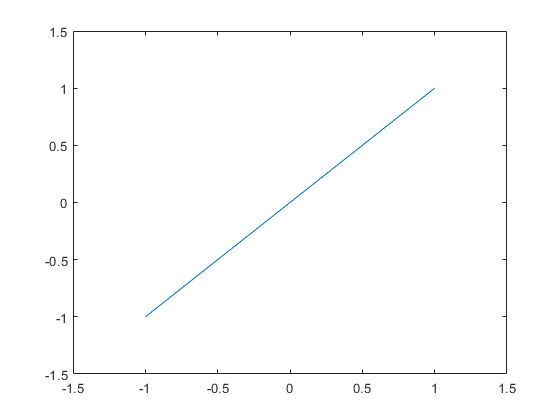
\includegraphics[width=0.5\textwidth]{images/01a.png}
    \caption{$x = 1,~vx = 0,~y = +1, vy = 0$}
\end{figure}

\begin{figure}[H]
\centering
    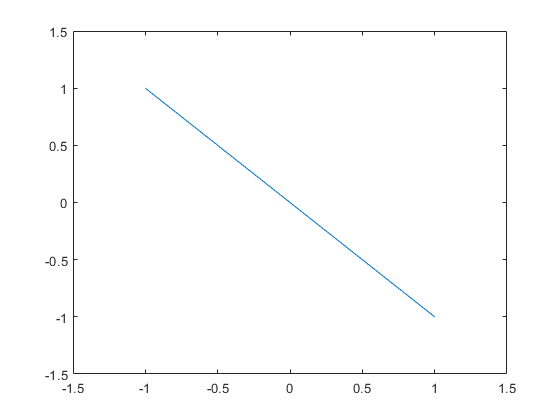
\includegraphics[width=0.5\textwidth]{images/01b.png}
    \caption{$x = 1,~vx = 0,~y = -1, vy = 0$}
\end{figure}

\begin{figure}[H]
\centering
    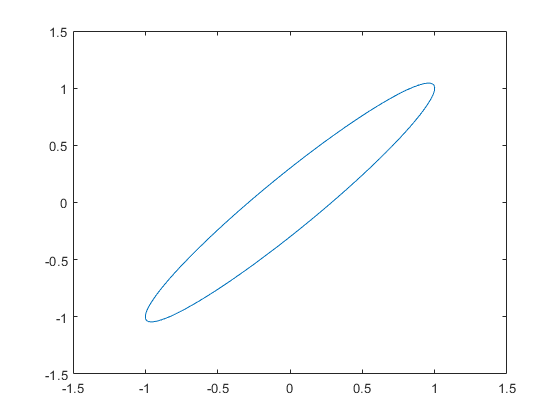
\includegraphics[width=0.5\textwidth]{images/01c.png}
    \caption{$x = 1,~vx = 0,~y = +1, vy = 0.3$}
\end{figure}

\begin{figure}[H]
\centering
    \includegraphics[width=0.5\textwidth]{images/01D.png}
    \caption{$x = 1,~vx = 0,~y = -1, vy = 0.3$}
\end{figure}

\begin{figure}[H]
\centering
    \includegraphics[width=0.5\textwidth]{images/01E.png}
    \caption{$x = 1,~vx = 0,~y = 0, vy = 0.3$}
\end{figure}

\section{Ejercicio 2}

Utilizaremos el siguiente código para desarrollar las gráficas correspondientes, con los cambios tanto para $l$ y para $n$, en el mismo orden de las condiciones del anterior ejercicio.
\begin{lstlisting} [frame=single]
clear; clf; hold off; n=0; h=0.0001;
% Constantes del Sistema
 m1=1; l=1; k1=m1*l^2;
% Constantes para cambiar
 m2=1; n=1; k2=m2*n^2;
% Condiciones Iniciales
x = 1; vx = 0; y = 1; vy = 0;
ax = -k1*x/m1;  
ay = -k2*y/m2; 
tfin=100; n=0;
% Inicio de la Simulacion
px(1)=x; py(1)=y;
for t=0:h:tfin
    n  = n+1;
    ax =-k1*x/m1;
    vx = vx + ax*h;
    x  = x  + vx*h;
    ay =-k2*y/m2;
    vy = vy + ay*h;
    y  = y  + vy*h;
    px(n+1)=x;
    py(n+1)=y;
end
subplot(4,2,1)
plot(px,py)
title('l = 1 y n = 1')
%%%%%%%%%%%%%%%%%%
m1=1; l=1; k1=m1*l^2;
m2=2; n=2; k2=m2*n^2;
x = 1; vx = 0; y = 1; vy = 0;
ax = -k1*x/m1;  
ay = -k2*y/m2; 
tfin=100; n=0;
% Inicio de la Simulacion
px(1)=x; py(1)=y;
for t=0:h:tfin
    n  = n+1;
    ax =-k1*x/m1;
    vx = vx + ax*h;
    x  = x  + vx*h;
    ay =-k2*y/m2;
    vy = vy + ay*h;
    y  = y  + vy*h;
    px(n+1)=x;
    py(n+1)=y;
end
subplot(4,2,2)
plot(px,py)
title('l = 1 y n = 2')
%%%%%%%%%%%%%%%%%%
m1=1; l=1; k1=m1*l^2;
m2=1; n=3; k2=m2*n^2;
x = 1; vx = 0; y = 1; vy = 0;
ax = -k1*x/m1;  
ay = -k2*y/m2; 
tfin=100; n=0;
px(1)=x; py(1)=y;
for t=0:h:tfin
    n  = n+1;
    ax =-k1*x/m1;
    vx = vx + ax*h;
    x  = x  + vx*h;
    ay =-k2*y/m2;
    vy = vy + ay*h;
    y  = y  + vy*h;
    px(n+1)=x;
    py(n+1)=y;
end
subplot(4,2,3)
plot(px,py)
title('l = 1 y n = 3')
%%%%%%%%%%%%%%%%%%
m1=1; l=2; k1=m1*l^2;
m2=1; n=3; k2=m2*n^2;
x = 1; vx = 0; y = 1; vy = 0;
ax = -k1*x/m1;  
ay = -k2*y/m2; 
tfin=100; n=0;
px(1)=x; py(1)=y;
for t=0:h:tfin
    n  = n+1;
    ax =-k1*x/m1;
    vx = vx + ax*h;
    x  = x  + vx*h;
    ay =-k2*y/m2;
    vy = vy + ay*h;
    y  = y  + vy*h;
    px(n+1)=x;
    py(n+1)=y;
end
subplot(4,2,4)
plot(px,py)
title('l = 2 y n = 3')
%%%%%%%%%%%%%%%%%%
m1=1; l=3; k1=m1*l^2;
m2=1; n=4; k2=m2*n^2;
x = 1; vx = 0; y = 1; vy = 0;
ax = -k1*x/m1;  
ay = -k2*y/m2; 
tfin=100; n=0;
px(1)=x; py(1)=y;
for t=0:h:tfin
    n  = n+1;
    ax =-k1*x/m1;
    vx = vx + ax*h;
    x  = x  + vx*h;
    ay =-k2*y/m2;
    vy = vy + ay*h;
    y  = y  + vy*h;
    px(n+1)=x;
    py(n+1)=y;
end
subplot(4,2,5)
plot(px,py)
title('l = 3 y n = 4')
%%%%%%%%%%%%%%%%%%
m1=1; l=3; k1=m1*l^2;
m2=1; n=5; k2=m2*n^2;
x = 1; vx = 0; y = 1; vy = 0;
ax = -k1*x/m1;  
ay = -k2*y/m2; 
tfin=100; n=0;
px(1)=x; py(1)=y;
for t=0:h:tfin
    n  = n+1;
    ax =-k1*x/m1;
    vx = vx + ax*h;
    x  = x  + vx*h;
    ay =-k2*y/m2;
    vy = vy + ay*h;
    y  = y  + vy*h;
    px(n+1)=x;
    py(n+1)=y;
end
subplot(4,2,6)
plot(px,py)
title('l = 3 y n = 5')
%%%%%%%%%%%%%%%%%%
m1=1; l=4; k1=m1*l^2;
m2=1; n=5; k2=m2*n^2;
x = 1; vx = 0; y = 1; vy = 0;
ax = -k1*x/m1;  
ay = -k2*y/m2; 
tfin=100; n=0;
px(1)=x; py(1)=y;
for t=0:h:tfin
    n  = n+1;
    ax =-k1*x/m1;
    vx = vx + ax*h;
    x  = x  + vx*h;
    ay =-k2*y/m2;
    vy = vy + ay*h;
    y  = y  + vy*h;
    px(n+1)=x;
    py(n+1)=y;
end
subplot(4,2,7)
plot(px,py)
title('l = 4 y n = 5')
%%%%%%%%%%%%%%%%%%
m1=1; l=5; k1=m1*l^2;
m2=1; n=6; k2=m2*n^2;
x = 1; vx = 0; y = 1; vy = 0;
ax = -k1*x/m1;  
ay = -k2*y/m2; 
tfin=100; n=0;
px(1)=x; py(1)=y;
for t=0:h:tfin
    n  = n+1;
    ax =-k1*x/m1;
    vx = vx + ax*h;
    x  = x  + vx*h;
    ay =-k2*y/m2;
    vy = vy + ay*h;
    y  = y  + vy*h;
    px(n+1)=x;
    py(n+1)=y;
end
subplot(4,2,8)
plot(px,py)
title('l = 5 y n = 6')
\end{lstlisting}

\begin{figure}[H]
\centering
    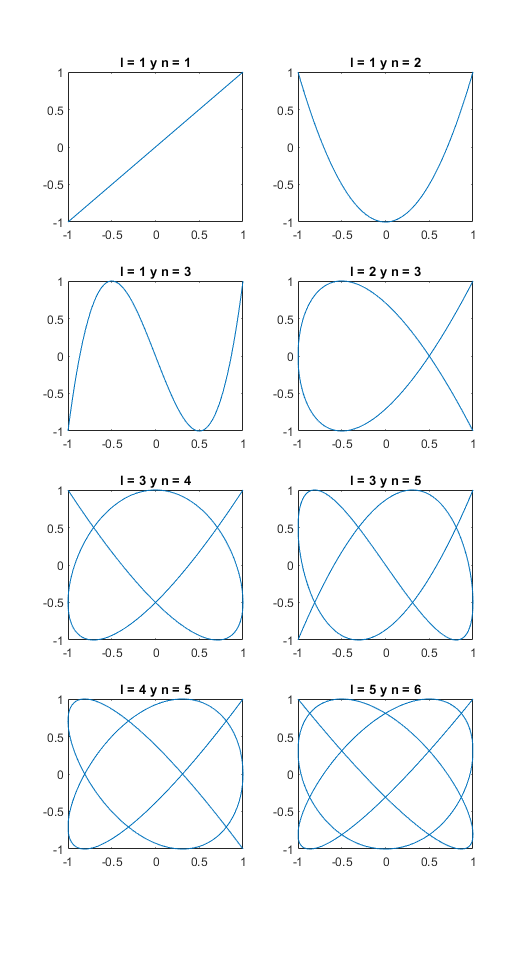
\includegraphics[width=0.6\textwidth]{images/02a.png}
    \caption{$x = 1,~vx = 0,~y = +1, vy = 0$}
\end{figure}

\begin{figure}[H]
\centering
    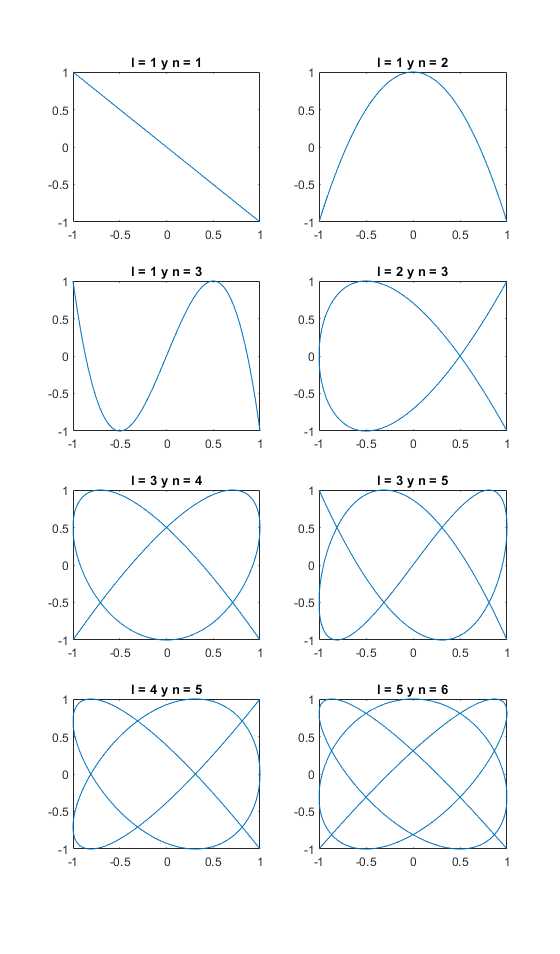
\includegraphics[width=0.7\textwidth]{images/02b.png}
    \caption{$x = 1,~vx = 0,~y = -1, vy = 0$}
\end{figure}

\begin{figure}[H]
\centering
    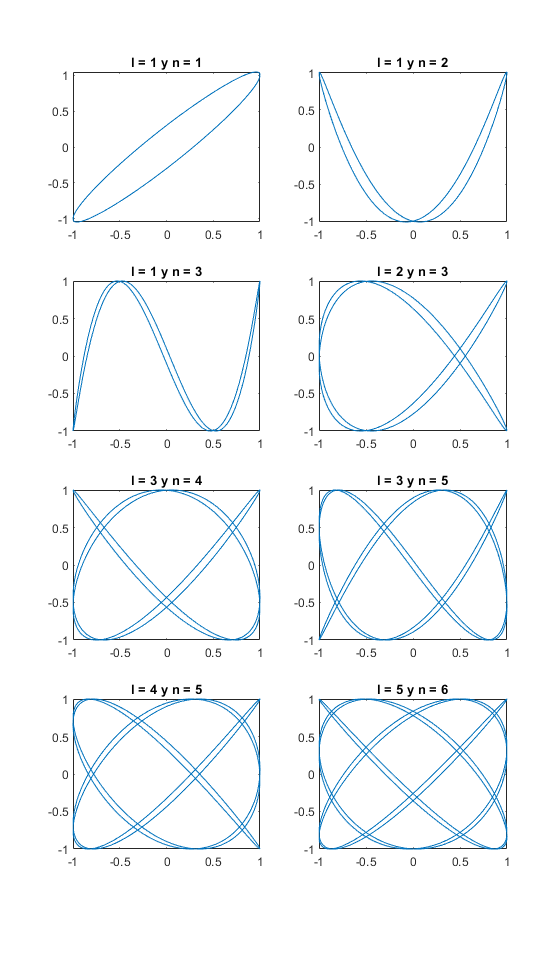
\includegraphics[width=0.7\textwidth]{images/02c.png}
    \caption{$x = 1,~vx = 0,~y = +1, vy = 0.3$}
\end{figure}

\begin{figure}[H]
\centering
    \includegraphics[width=0.7\textwidth]{images/02D.png}
    \caption{$x = 1,~vx = 0,~y = -1, vy = 0.3$}
\end{figure}

\begin{figure}[H]
\centering
    \includegraphics[width=0.7\textwidth]{images/02E.png}
    \caption{$x = 1,~vx = 0,~y = 0, vy = 0.3$}
\end{figure}

\section{Ejercicio 3}

Para el desarrollo del ejercicio 3 se utilizó el sigueinte código, de la misma forma se cambiarán los datos para generar las diferentes gráficas.

\begin{lstlisting} [frame=single]
clear; clf; hold off; n=0; h=0.0001;

cM = [1 1 1; 1 1 2; 1 1 3; 1 2 3; 1 2 2; 2 3 3; 3 5 6; 4 4 4; 5 6 7]
cC = 1
for t=1:1:9
    cM(t,1);
    cM(t,2);
    cM(t,3);
    % Constantes del Sistema
    m1=1; l=cM(t,1); k1=m1*l^2;
    % Constantes para cambiar
    m2=1; n=cM(t,2); k2=m2*n^2;
    m3=1; p=cM(t,3); k3=m3*p^2;
    n2 = n
    % Condiciones Iniciales
    x = 1; vx = 0; z = 1; vz = 0; y = 1; vy = 0;
    ax = -k1*x/m1;  
    ay = -k2*y/m2; 
    az = -k3*z/m3; 
    tfin=100; n=0;
    % Inicio de la Simulacion
    px(1)=x; py(1)=y; pz(1)=z;
    for t=0:h:tfin
        n  = n+1;
        ax =-k1*x/m1;
        vx = vx + ax*h;
        x  = x  + vx*h;
        ay =-k2*y/m2;
        vy = vy + ay*h;
        y  = y  + vy*h;
        az =-k3*z/m3;
        vz = vz + az*h;
        z  = z  + vz*h;
        px(n+1)=x;
        py(n+1)=y;
        pz(n+1)=z;
    end
    subplot(3,3,cC)
    plot3(px,py,pz)
    xlabel('X');
    ylabel('Y');
    zlabel('Z');
    title([num2str(l),' : ',num2str(n2), ' : ',num2str(p)])
    grid on;
    cC = cC + 1;
end
\end{lstlisting}

%%%%%%%%%%%%%%%%%%%%%%%%%%%%%%%%%%%%%%%%%%%%%%%%%%%%%%%%%%%%%%%%%%1
\clearpage
\newpage

\begin{figure}
\centering
    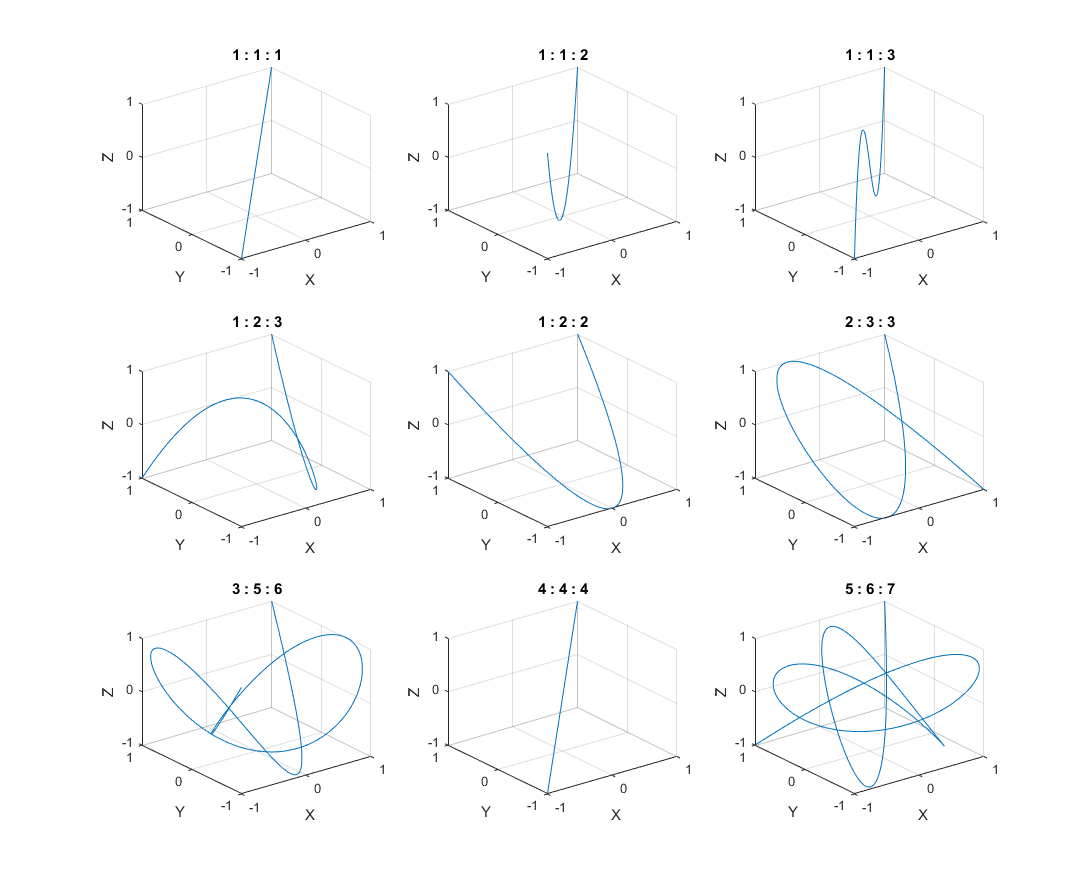
\includegraphics[width=1\textwidth]{images/03a1.png}
    \caption{$x = 1,~vx = 0,~z = 1,~vz = 0,~y = 1,~vy = 0$}
\end{figure}

\clearpage
\newpage

\begin{figure}
\centering
    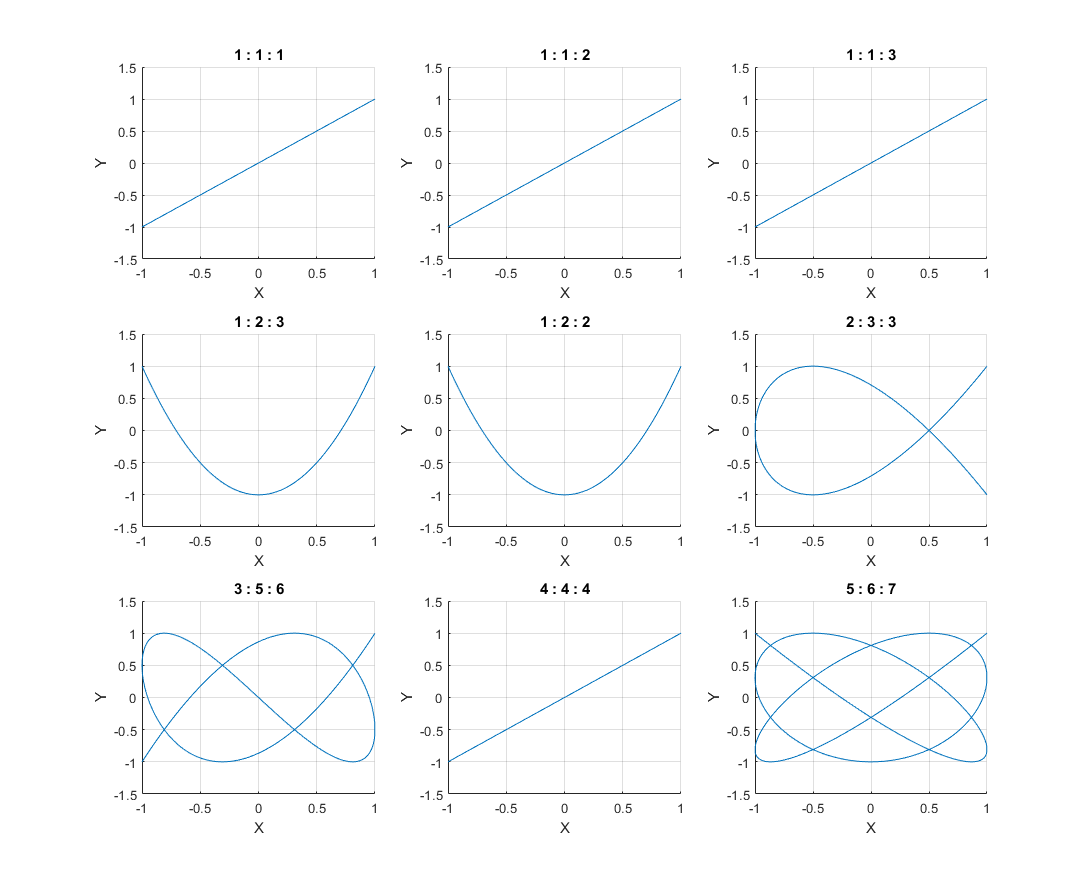
\includegraphics[width=1\textwidth]{images/03a2.png}
    \caption{$x = 1,~vx = 0,~z = 1,~vz = 0,~y = 1,~vy = 0$ con ubicación en los ejes $x$ e $y$}
\end{figure}

%%%%%%%%%%%%%%%%%%%%%%%%%%%%%%%%%%%%%%%%%%%%%%%%%%%%%%%%%%%%%%%%%2
\clearpage
\newpage

\begin{figure}
\centering
    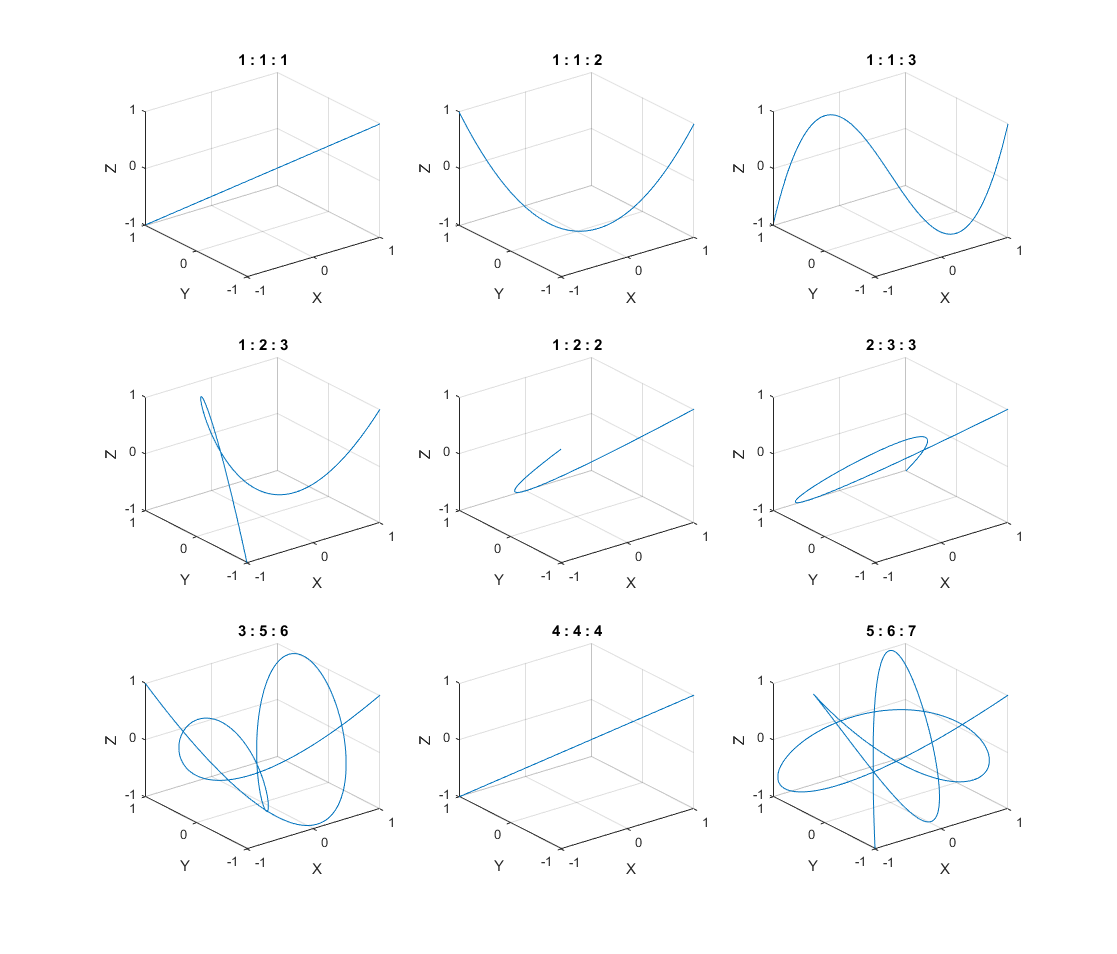
\includegraphics[width=1\textwidth]{images/03b1.png}
    \caption{$x = 1,~vx = 0,~z = 1,~vz = 0,~y =-1,~vy = 0$}
\end{figure}

\clearpage
\newpage

\begin{figure}
\centering
    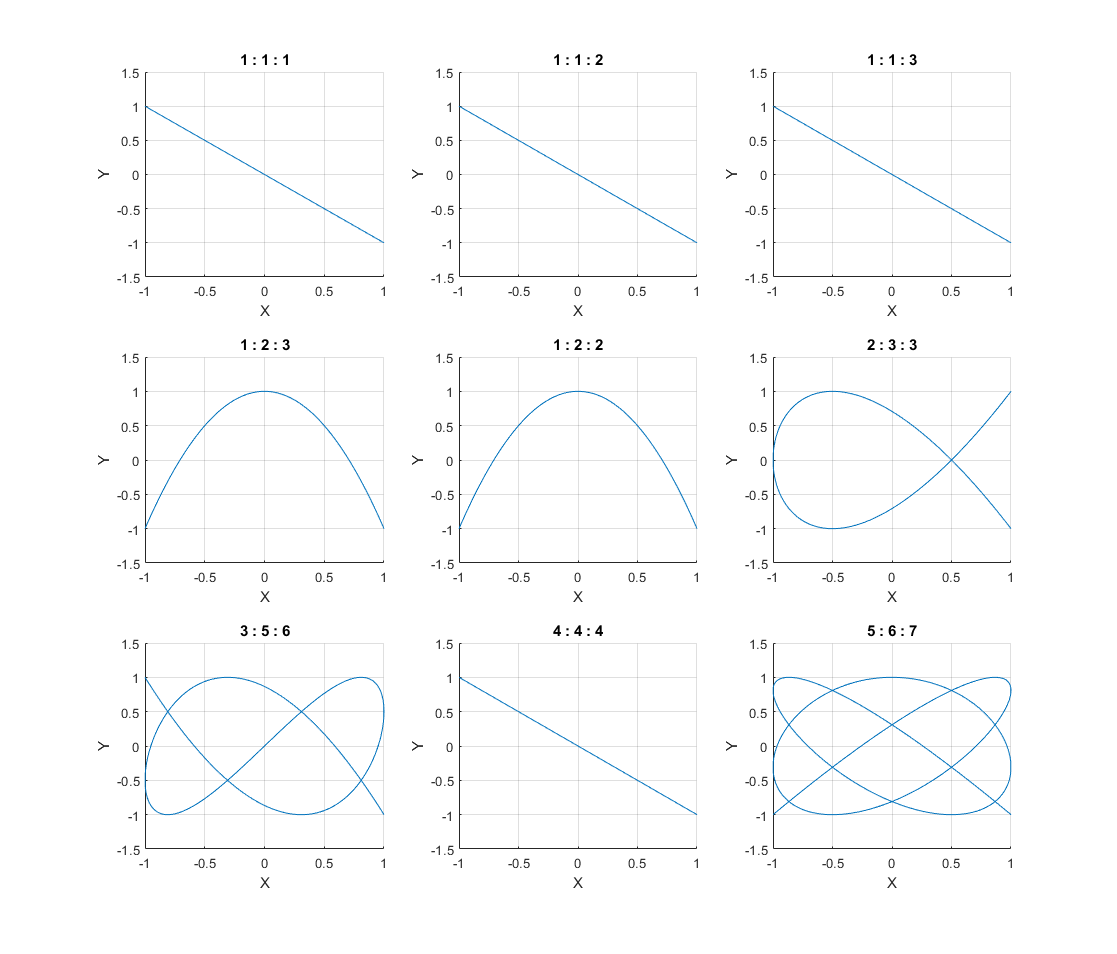
\includegraphics[width=1\textwidth]{images/03b2.png}
    \caption{$x = 1,~vx = 0,~z = 1,~vz = 0,~y =-1,~vy = 0$ con ubicación en los ejes $x$ e $y$}
\end{figure}

%%%%%%%%%%%%%%%%%%%%%%%%%%%%%%%%%%%%%%%%%%%%%%%%%%%%%%%%%%%%%%%%%3
\clearpage
\newpage

\begin{figure}
\centering
    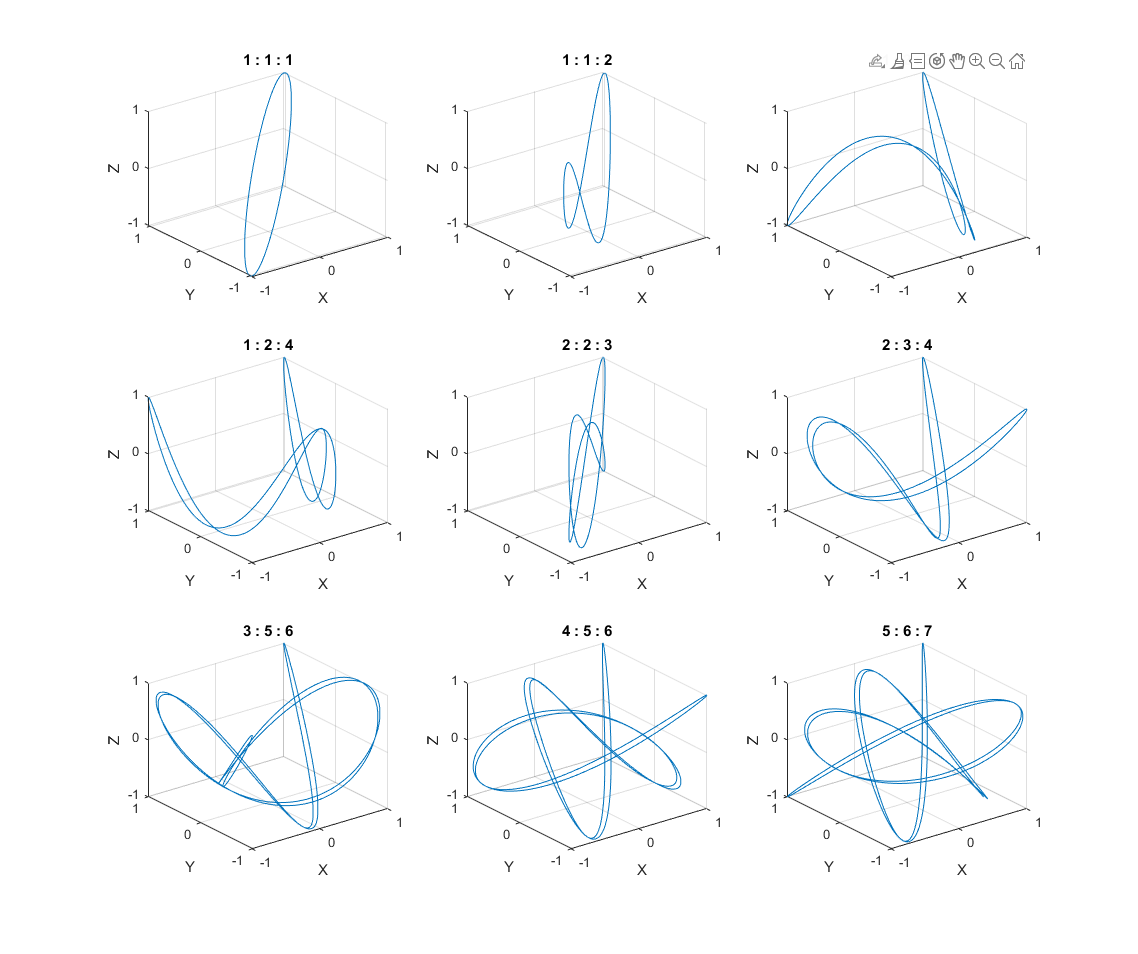
\includegraphics[width=1\textwidth]{images/03c1.png}
    \caption{$x = 1,~vx = 0,~z = 1,~vz = 0,~y = 1,~vy = 0.3$}
\end{figure}

\clearpage
\newpage

\begin{figure}
\centering
    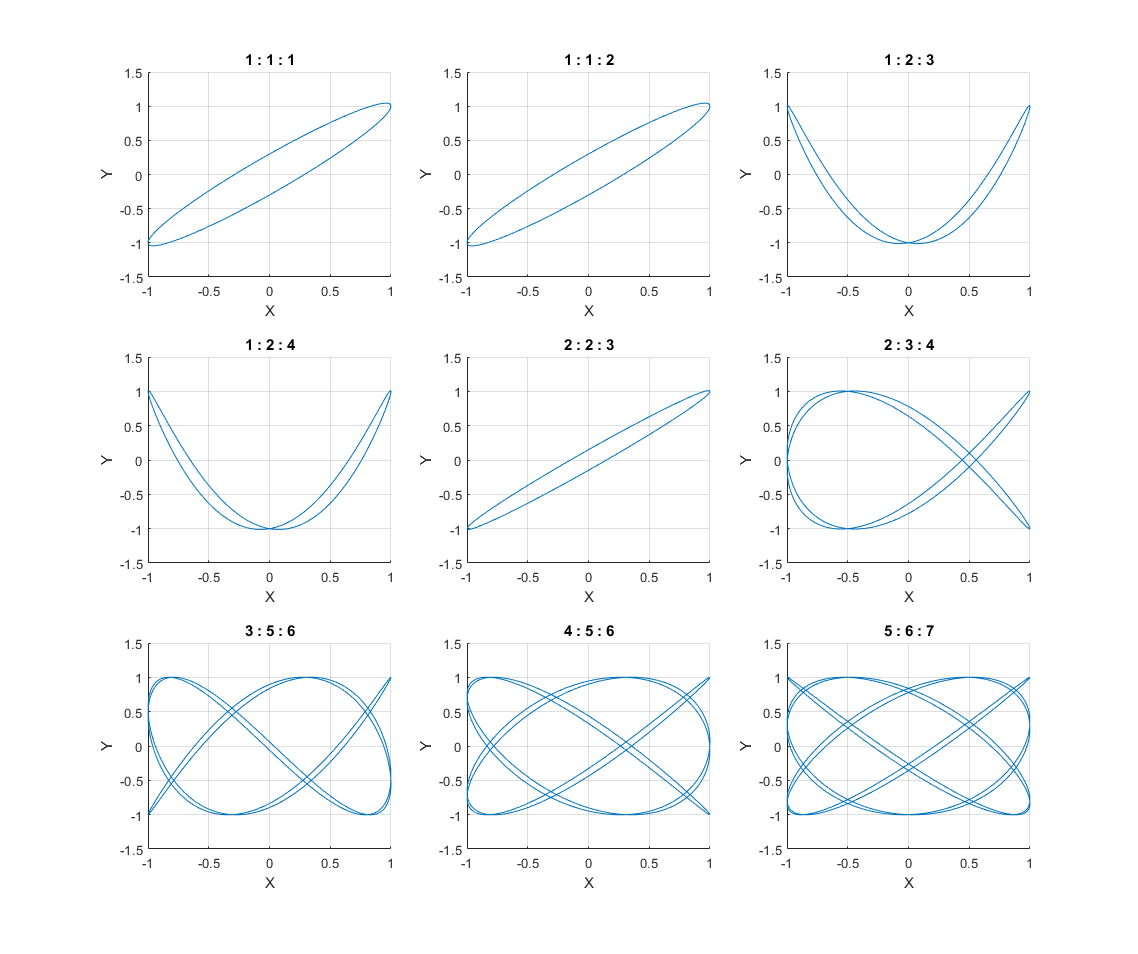
\includegraphics[width=1\textwidth]{images/03c2.png}
    \caption{$x = 1,~vx = 0,~z = 1,~vz = 0,~y =-1,~vy = 0.3$ con ubicación en los ejes $x$ e $y$}
\end{figure}

%%%%%%%%%%%%%%%%%%%%%%%%%%%%%%%%%%%%%%%%%%%%%%%%%%%%%%%%%%%%%%%%%4
\clearpage
\newpage

\begin{figure}
\centering
    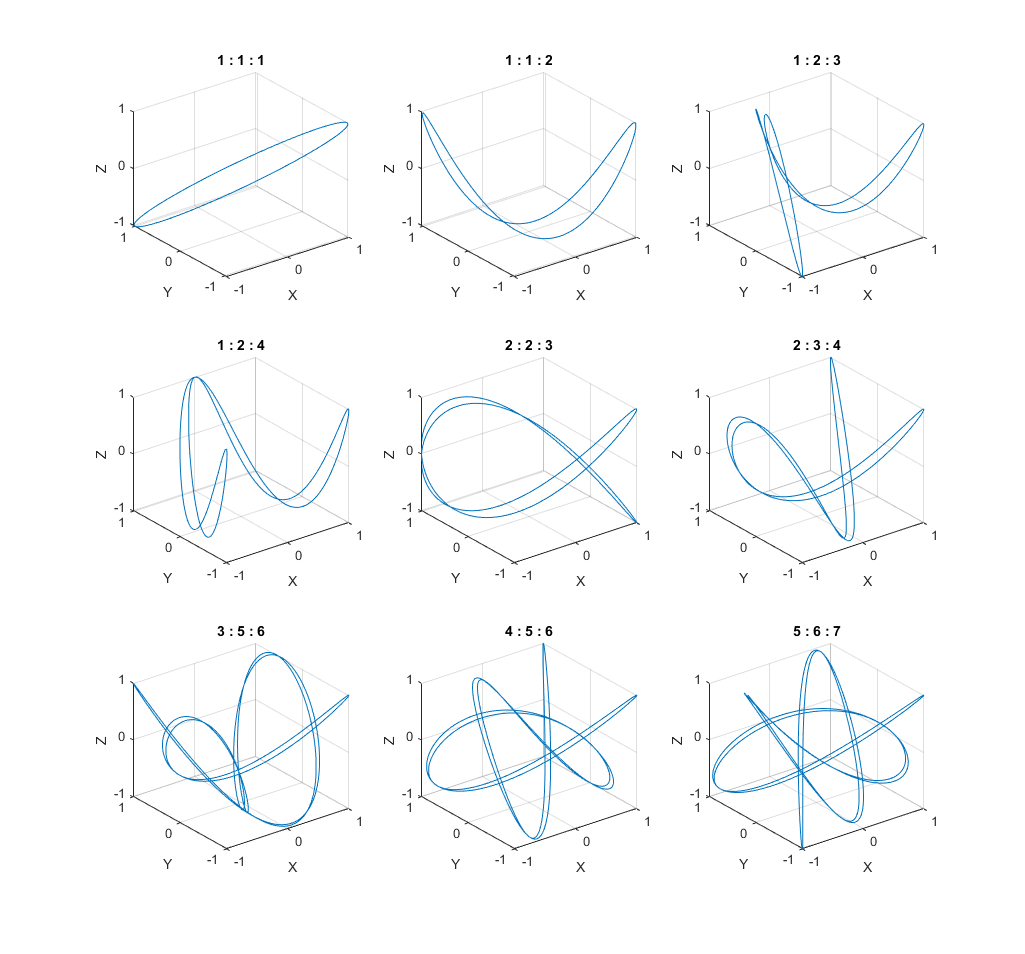
\includegraphics[width=1\textwidth]{images/03d1.png}
    \caption{$x = 1,~vx = 0,~z = 1,~vz = 0,~y =-1,~vy = 0$}
\end{figure}

\clearpage
\newpage

\begin{figure}
\centering
    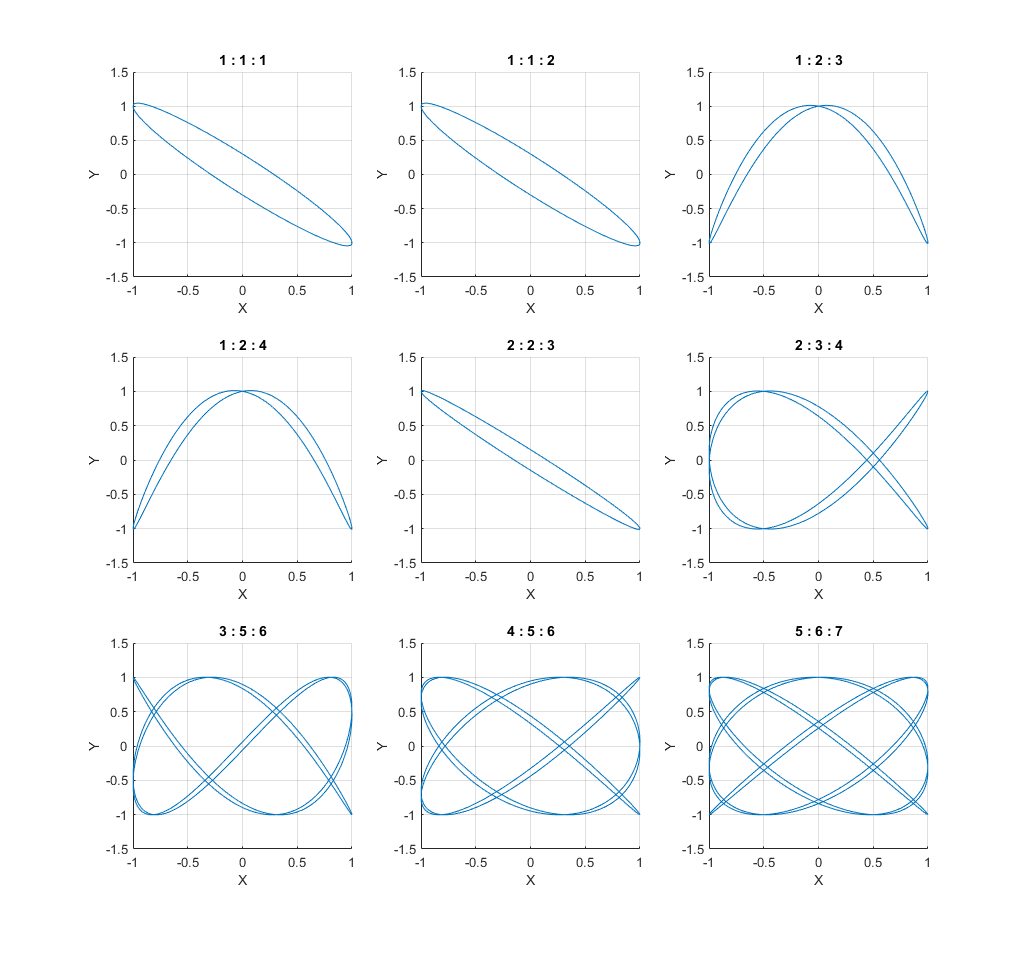
\includegraphics[width=1\textwidth]{images/03d2.png}
    \caption{$x = 1,~vx = 0,~z = 1,~vz = 0,~y = 0,~vy = 0.3$ con ubicación en los ejes $x$ e $y$}
\end{figure}

%%%%%%%%%%%%%%%%%%%%%%%%%%%%%%%%%%%%%%%%%%%%%%%%%%%%%%%%%%%%%%%%%5
\clearpage
\newpage

\begin{figure}
\centering
    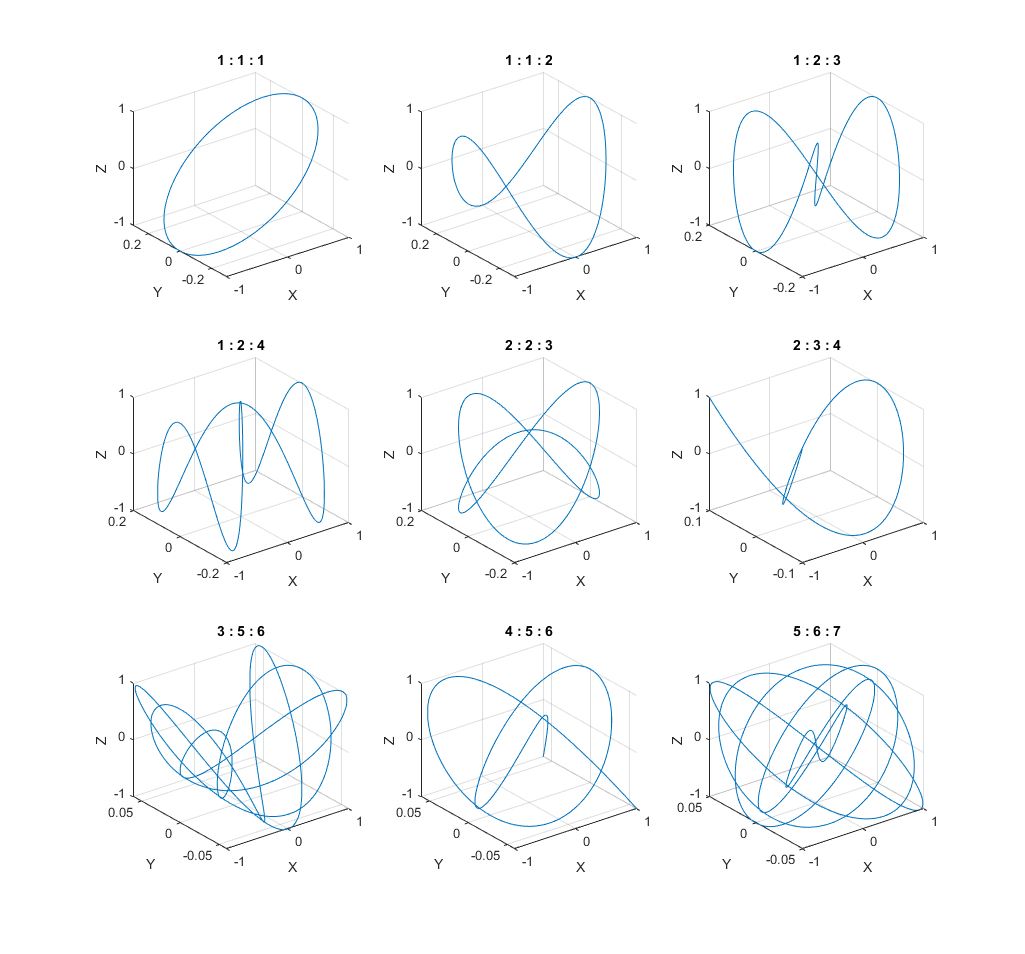
\includegraphics[width=1\textwidth]{images/03e1.png}
    \caption{$x = 1,~vx = 0,~z = 1,~vz = 0,~y =-1,~vy = 0$}
\end{figure}

\clearpage
\newpage

\begin{figure}
\centering
    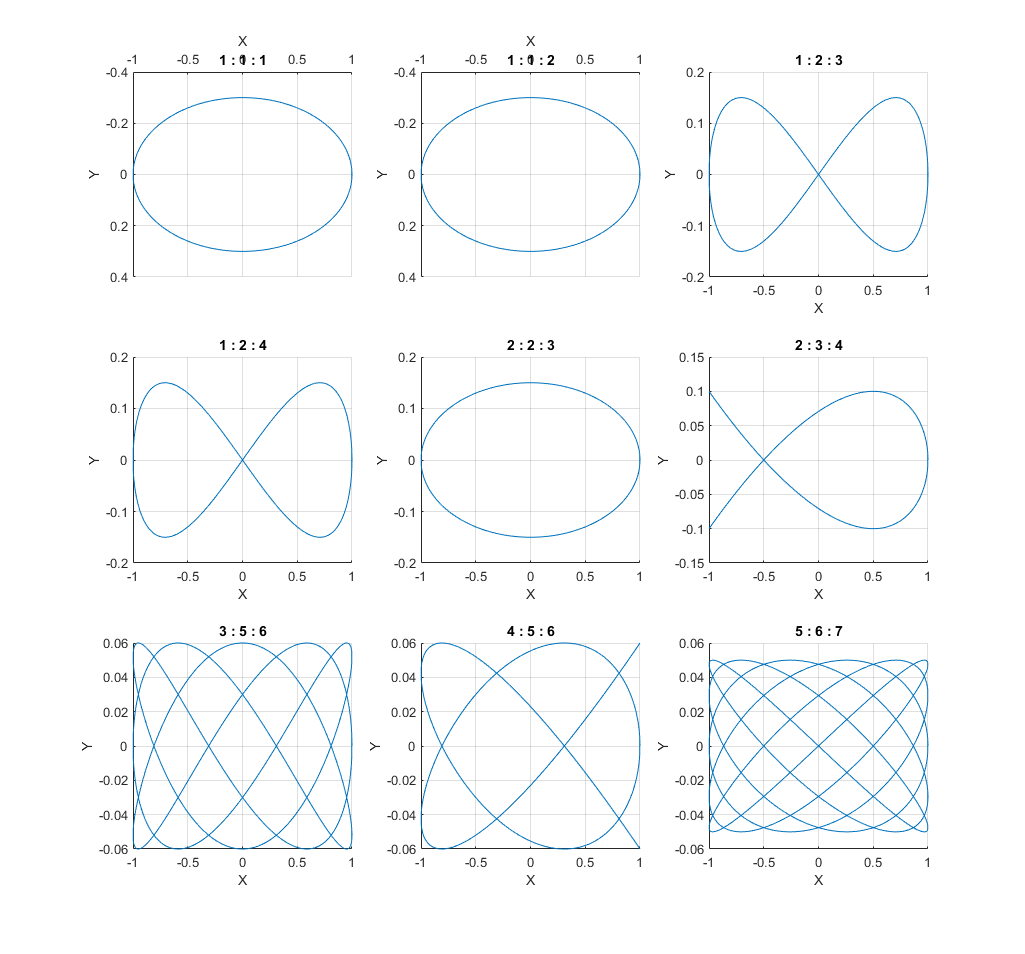
\includegraphics[width=1\textwidth]{images/03e2.png}
    \caption{$x = 1,~vx = 0,~z = 1,~vz = 0,~y =-1,~vy = 0$ con ubicación en los ejes $x$ e $y$}
\end{figure}

\clearpage
\newpage

\section{Creación del GIF}

Para la creación del .gif se utilizó el siguiente código, así como podemos verlo en \textcolor{blue}{
    \href{https://drive.google.com/file/d/18ty9yVBC-cS93bjtITK4pBOQUVgsb4mP/view?usp=sharing}{Gif}}.

\begin{lstlisting} [frame=single]
clear; clf; hold off; n=0; h=0.01;

    % Constantes del Sistema
    m1=1; l=5; k1=m1*l^2;
    % Constantes para cambiar
    m2=1; n=6; k2=m2*n^2;
    n2 = n;
    m3=1; p=7; k3=m3*p^2;
    % Condiciones Iniciales
    x = 1; vx = 0; z = 1; vz = 0; y = 0; vy = 0.3;
    ax = -k1*x/m1;  
    ay = -k2*y/m2; 
    az = -k3*z/m3; 
    tfin=10; n=0;
    % Inicio de la Simulacion
    px(1)=x; py(1)=y; pz(1)=z;
    drawnow;
    frame = getframe(1);
    im = frame2im(frame);        
    [imind,cm] = rgb2ind(im,256);       
    outfile = 'lissajous3DCarlosMestas.gif';
    imwrite(imind,cm,outfile,'gif','DelayTime',0,'loopcount',inf);      

    for t=0:h:tfin
        n  = n+1;
        ax =-k1*x/m1;
        vx = vx + ax*h;
        x  = x  + vx*h;
        ay =-k2*y/m2;
        vy = vy + ay*h;
        y  = y  + vy*h;
        az =-k3*z/m3;
        vz = vz + az*h;
        z  = z  + vz*h;
        px(n+1)=x;
        py(n+1)=y;
        pz(n+1)=z;  
        drawnow;
        frame = getframe(1);
        im = frame2im(frame);        
        [imind,cm] = rgb2ind(im,256);       
        imwrite(imind,cm,outfile,'gif','DelayTime',0,'writemode','append');
        plot3(px,py,pz)
        xlabel('X');
        ylabel('Y');
        zlabel('Z');
        title([num2str(l),' : ',num2str(n2), ' : ',num2str(p)])
%         pause(0.00000001)
        grid on;  
    end
\end{lstlisting}

\begin{figure}[H]
\centering
    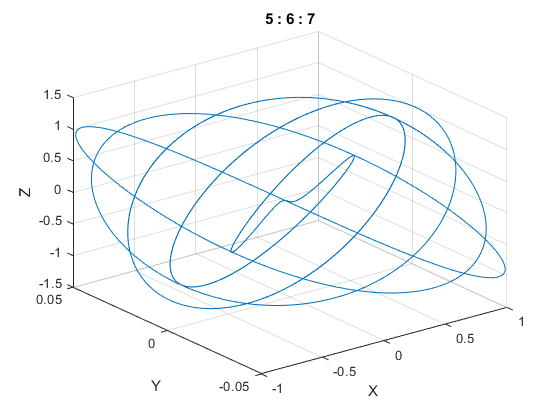
\includegraphics[width=0.7\textwidth]{images/gif3DImage1.png}
    \caption{Imagen del gif creado}
\end{figure}

\begin{figure}[H]
\centering
    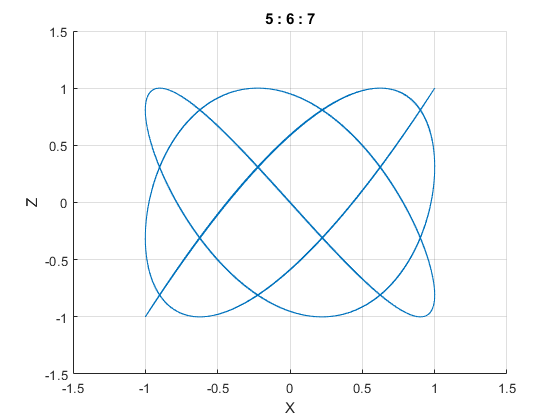
\includegraphics[width=0.7\textwidth]{images/gif3DImage2.png}
    \caption{Vista de los ejes $x$ y $z$}
\end{figure}

\begin{figure}[H]
\centering
    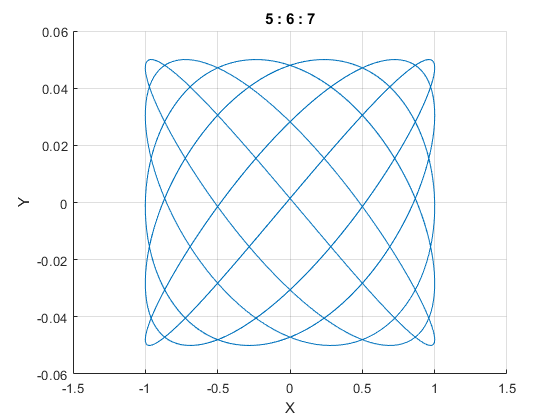
\includegraphics[width=0.7\textwidth]{images/gif3DImage3.png}
    \caption{Vista de los ejes $x$ e $y$}
\end{figure}

\begin{figure}[H]
\centering
    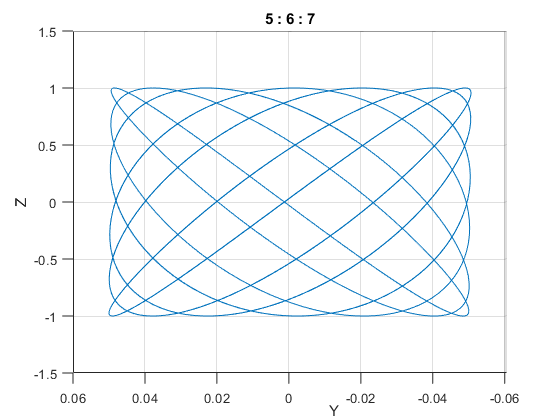
\includegraphics[width=0.7\textwidth]{images/gif3DImage4.png}
    \caption{Vista de los ejes $y$ y $z$}
\end{figure}


\end{document}